\subsection{Residual map and principal unresolved comparisons}

The residuals for the restricted six-row table are shown in \Cref{fig:residual-plot}. The carrier-linked electromagnetic, birefringence, and baryon-density channels all remain within the displayed few-sigma window. The CKM phase is not plotted here because it is better treated, at present, as the main unresolved transport-side comparison and is therefore moved to Appendix~\ref{app:benchmarks}.

\begin{figure}[t]
\centering
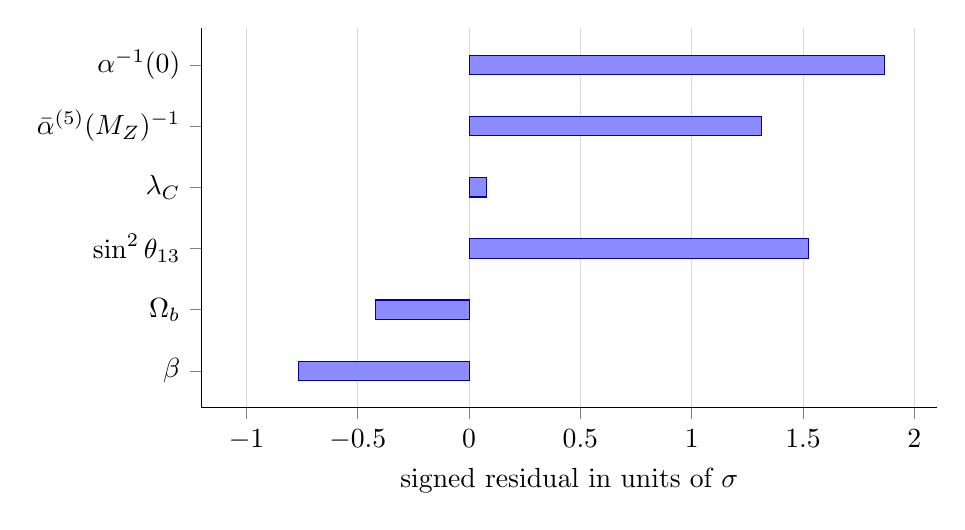
\begin{tikzpicture}
\begin{axis}[
    width=0.9\linewidth,
    height=6.4cm,
    xbar,
    bar width=7pt,
    xmin=-1.2,
    xmax=2.1,
    xlabel={signed residual in units of $\sigma$},
    symbolic y coords={beta,omegab,theta13,lambdac,alphaMZ,alpha0},
    ytick=data,
    yticklabels={$\beta$,$\Omega_b$,$\sin^2\theta_{13}$,$\lambda_C$,$\bar\alpha^{(5)}(M_Z)^{-1}$,$\alpha^{-1}(0)$},
    enlarge y limits=0.12,
    axis x line*=bottom,
    axis y line*=left,
    tick align=outside,
    major grid style={draw=gray!30},
    xmajorgrids=true
]
\addplot[fill=blue!45, draw=blue!70!black] coordinates {
    (-0.768,beta)
    (-0.421,omegab)
    (1.524,theta13)
    (0.078,lambdac)
    (1.315,alphaMZ)
    (1.865,alpha0)
};
\end{axis}
\end{tikzpicture}
\caption{Residual plot for the main benchmark rows with declared uncertainties.}
\label{fig:residual-plot}
\end{figure}

The principal unresolved comparisons are therefore specific rather than diffuse:
\begin{itemize}[leftmargin=1.5em, topsep=3pt, itemsep=2pt]
    \item the CKM phase needs either a genuine discrete derivation or a cleaner statement that the current relation is only a transport bridge,
    \item the bosonic relative index remains the decisive geometric theorem for the Higgs sector,
    \item the $\chi$-channel heat-kernel closure must be shown in one declared scheme before the induced-Einstein narrative can be treated as more than a coherent target.
\end{itemize}

\subsection{Falsification matrix}

\begin{table}[t]
\centering
\small
\begin{tabularx}{\linewidth}{@{}>{\raggedright\arraybackslash}p{0.24\linewidth}YY>{\raggedright\arraybackslash}p{0.13\linewidth}@{}}
\toprule
Statement & What would falsify it & Sector affected & Local or global failure \\
\midrule
Minimal carrier $E_3\oplus E_2$ & failure to recover the one-family packet or the global quotient from the carrier theorem & Hard & global \\
Family bridge and $\Oadm=48$ & no geometric monodromy interpretation of the three-cycle family space & Bridge & local-to-structural \\
Bosonic relative index selecting $\Phi$ & no unique seam-even doublet or an unavoidable extra light triplet & Completion & local \\
$\chi$-channel Einstein bridge & inability to obtain one common closure for $\Mpl$, $v$, and the comparison map & Completion & global \\
Transport positivity and strong CP closure & nonzero determinant phase or an unavoidable $\bar\theta$ counterterm & Completion & local \\
Confinement as admissible word selection & necessity of physical states with $z(w)\neq1$ in the low-energy spectrum & Completion & local \\
\bottomrule
\end{tabularx}
\caption{Falsification matrix for the present main-paper claims.}
\label{tab:falsification}
\end{table}

\section{Conditional master theorem and finite proof obligations}

\subsection{Compiler chain}

Collecting the present hard, bridge, and completion layers, the intended compiler line is
\begin{equation}
\label{eq:conditional-compiler-chain}
\begin{aligned}
(\widetilde M\to M,\Seam,\inv,\chi)
&\Rightarrow
(E_3\oplus E_2,\ G_{\SM}^{\mathrm{glob}},\ S^+)\\
&\Rightarrow
(N_{\mathrm{fam}}=3,\ \Oadm=48,\ F,\ \Phi)\\
&\Rightarrow
(\Mpl,\ v,\ \mathcal Y_f,\ \sigma,\ \bar\theta)\\
&\Rightarrow
(m_f,\ V_{\mathrm{CKM}},\ U_{\mathrm{PMNS}},\ \text{hadrons})\\
&\Rightarrow
(\text{benchmarks},\ \Pred).
\end{aligned}
\end{equation}
This line is not meant as a slogan. Each arrow is attached either to a hard theorem, a bridge construction, or one of the explicit completion interfaces listed in the proof-obligation table below.

\subsection{Conditional master theorem}

\begin{theorem}[Conditional master theorem]
Assume the hard carrier and kernel layers summarized in \Cref{tab:status-matrix}, together with the completion statements of the geometric and transport programs and the declared comparison map $\mathcal R_{\SM}$. Then every observable in the present main-text scope is the output of one carrier-first relative spectral compiler from primitive seam data to scheme-specified observables.
\end{theorem}

\begin{proof}[Proof sketch]
The proof is compositional. The hard layer fixes the carrier, the global Standard Model quotient, one family, the carrier norm, the abelian index, and the established electromagnetic kernel. The bridge layer lifts the carrier packet to family multiplicity and occupancy and installs the RG/comparison interface. The completion layer is then finite: a bosonic relative index is asked to select the unique light Higgs mode, the $\chi$ channel is asked to produce $\Mpl$ and $v$, the phase-distance transport kernel is asked to generate Yukawas and mixings, and center-neutral admissibility is asked to close confinement and strong CP. Once these completion arrows are granted, no further primitive category is needed for the particle, mass, and benchmark compiler described here.
\end{proof}

\subsection{Finite proof obligations}

\begin{table}[t]
\centering
\small
\begin{tabularx}{\linewidth}{@{}>{\raggedright\arraybackslash}p{0.20\linewidth}>{\raggedright\arraybackslash}p{0.18\linewidth}>{\raggedright\arraybackslash}p{0.20\linewidth}YY@{}}
\toprule
Target statement & Input data & Missing lemma & Minimal deliverable & Empirical consequence \\
\midrule
Family space theorem & $\Seam$, $C_1,C_2,C_T$, $T^3=1$ & monodromy-to-family theorem & derive $F$ from the seam cycle algebra & stabilizes the meaning of $\Oadm=48$ \\
Bosonic index closure & $E_3\oplus E_2$, $\mathcal B_{\mathrm{rel}}$ & relative bosonic index theorem & prove unique seam-even doublet selection & Higgs-sector hardening \\
$\chi$-channel closure & $\mathbb A_{\Seam}$, APS data, heat-kernel coefficients & relative heat-kernel computation & explicit coefficient map with declared scheme & Planck / Higgs bridge becomes testable \\
Transport distance theorem & $U_6$, $D_y$, admissible words & phase-distance theorem & derive $L_{f,j}$ and bounded $\Lambda_{f,j}$ from transport geometry & CKM / PMNS and mass hierarchy become sharper \\
Comparison bridge & $\alpha(0)$, $\Omega_b$, $\beta$, scheme map $\mathcal R_{\SM}$ & RG and matching control & one declared threshold / scheme section & quantitative theory-versus-data map becomes convention-complete \\
\bottomrule
\end{tabularx}
\caption{Finite proof obligations for the present main-paper form.}
\label{tab:proof-obligations}
\end{table}

\section{Conclusion}

The present paper argues that a small carrier-first core already fixes nontrivial physics: the minimal $3+2$ carrier, the global Standard Model quotient, one chiral family, the carrier norm $5/6$, the abelian index, the seam constant $\cthree$, the corrected opening $\phiz$, and the electromagnetic closure channel. The compression identities and exclusion theorems then show that this core is overdetermined: the rank-lock, the $41$-chain, the Cabibbo inversion, and the categorical failure of wrong discrete worlds are not additional ornaments but structural consequences of the same small algebra. What remains open is no longer a vague enlargement of the ontology, but a finite list of completion interfaces.

Those interfaces are explicit. The family local system must harden nondegeneracy and mixing; the family count itself is already supported by the local patch-deficit route. A bosonic relative index must select the unique light Higgs doublet. The $\chi$ channel must close the Planck and electroweak scales in one geometric response, with the Newton-form relation understood as a corollary rather than a second output. The transport kernel must harden Yukawas, mixings, confinement, and strong CP while separating positive radial mass data from unitary family holonomy cleanly enough that strong and weak CP are not conflated. The $\alpha$ row must remain tied to the full self-consistent solver rather than to a frozen opening. If those finite steps are completed, the same relative spectral framework yields one compiler from seam data to particle content, masses, hadronic admissibility, and scheme-specified observables. The open problem is therefore execution of a finite proof program, not addition of a new primitive layer.

\appendix

\section{Technical conventions and data layers}
\label{app:tech}

This appendix collects the technical bookkeeping that supports the carrier-first presentation but would slow the early main-text flow if placed before the carrier theorem.

\subsection{Relative objects}

The adjective \enquote{relative} is used in one fixed sense throughout the paper: every operator or action is compared to a declared reference object.

\begin{table}[t]
\centering
\small
\begin{tabularx}{\linewidth}{@{}>{\raggedright\arraybackslash}p{0.22\linewidth}YY@{}}
\toprule
Relative object & Definition or schematic form & Role \\
\midrule
$D_{\mathrm{rel}}$ & $D-D_{\mathrm{ref}}$ or a specified relative pair $(D,D_{\mathrm{ref}})$ & fermionic comparison operator \\
$S_{\mathrm{rel}}$ & $\tr f(D/\Lambda)-\tr f(D_{\mathrm{ref}}/\Lambda)+\frac{i\pi}{2}\Delta\eta$ & relative spectral action \\
$\Ind_{\mathrm{rel}}$ & APS-type index of a relative pair or superconnection package & carrier and bosonic counting \\
$\langle W(C)\rangle_{\mathrm{rel}}$ & Wilson observable after subtraction of the declared reference sector & confinement diagnostics \\
$\mathcal H_{\mathrm{rel}}$ & relative Hamiltonian used in admissible-sector minimization & optional record extension \\
\bottomrule
\end{tabularx}
\caption{Conventions on relative objects.}
\label{tab:relative-objects}
\end{table}

\subsection{Layered datum and admissibility}

\begin{construction}[Layered datum]
The technical bookkeeping behind the manuscript uses four levels:
\[
\Tcore
=
\bigl(
\widetilde M\to M,\ \Seam,\ \inv,\ D_{\mathrm{rel}},\ \mathsf{Adm}
\bigr),
\]
\[
\Tker
=
\bigl(
E_3\oplus E_2,\ Y,\ S^+,\ \gamma,\ B,\ G_{\SM}^{\mathrm{glob}},\ \bone(N_{\mathrm{fam}},N_\Phi)
\bigr),
\]
\[
\Tbridge
=
\bigl(
(F,T),\ \Oadm,\ \deltatop,\ \mathcal R_{\SM}
\bigr),
\]
\[
\Tcomp
=
\bigl(
(\chi,\mathcal B_{\mathrm{rel}},\mathbb A_{\Seam}),\ (U_6,D_y,\mathcal Y_y^{(\varepsilon)})
\bigr).
\]
\end{construction}

Conditional record, horizon, and prediction-semantics data are kept outside this compact layered datum and are introduced only in the dedicated appendix-level extension.

\begin{table}[t]
\centering
\small
\begin{tabularx}{\linewidth}{@{}>{\raggedright\arraybackslash}p{0.12\linewidth}>{\raggedright\arraybackslash}p{0.31\linewidth}>{\raggedright\arraybackslash}p{0.13\linewidth}Y@{}}
\toprule
Level & Objects & Claim role & Function in the present paper \\
\midrule
Core datum & $\widetilde M\to M$, $\Seam$, $\inv$, $D_{\mathrm{rel}}$, $\mathsf{Adm}$ & Hard & minimal input required to formulate admissibility and the carrier theorem \\
Carrier kernel & $E_3\oplus E_2$, $Y$, $S^+$, $\gamma$, $B$, $G_{\SM}^{\mathrm{glob}}$, $\bone(N_{\mathrm{fam}},N_\Phi)$ & Hard & rigid particle-theory packet extracted from the core datum \\
Bridge layer & $(F,T)$, $\Oadm$, $\deltatop$, $\mathcal R_{\SM}$ & Bridge & organizes family lift, occupancy, and scheme-specified comparison \\
Completion data & $(\chi,\mathcal B_{\mathrm{rel}},\mathbb A_{\Seam})$, $(U_6,D_y,\mathcal Y_y^{(\varepsilon)})$ & Completion & collects the open geometric and transport interfaces without promoting target outputs to primitive data \\
\bottomrule
\end{tabularx}
\caption{Core datum versus kernel, bridge, and completion structures.}
\label{tab:layered-datum}
\end{table}

\begin{definition}[Admissibility predicate]
In the present paper $\mathsf{Adm}$ denotes a predicate on relative sectors, and by mild abuse of notation also the induced class of admissible sectors. We write $\mathsf{Adm}(X)=1$ precisely when:
\begin{enumerate}[label=(\arabic*), leftmargin=1.5em, topsep=3pt, itemsep=2pt]
    \item $X$ lies in the declared domain of the relative operator pair,
    \item the associated relative action or index density is finite after reference subtraction,
    \item the required seam-evenness condition is satisfied,
    \item colored sectors satisfy center neutrality when a hadronic interpretation is intended,
    \item positivity and closure conditions hold in those sectors used for observable or transport statements.
\end{enumerate}
Thus $\mathsf{Adm}$ is not introduced here as a projector or a functor, but as a predicate that defines the class of sectors on which the later carrier, transport, and appendix-level constructions are allowed to act.
\end{definition}

\section{Constants atlas and downstream scale grammar}
\label{app:constants}

This appendix collects material that is useful for internal compression but should not dominate the main-text scope of explicit claims.

\subsection{Global rotation angle and constants atlas}

The seam loop is assumed to carry one unit of spectral flow,
\[
U_{\Seam}(\theta)=e^{i\theta},
\qquad
\SF(U_{\Seam})=1,
\qquad
\Delta_{\Seam}=2\pi.
\]
Because the spin lift closes only after $4\pi$, the normalized rotation modulus is
\[
\atheta=\frac{\theta}{4\pi}.
\]
The cascade in \Cref{fig:constant-cascade} is kept here as technical bookkeeping rather than as an early main-text dependency graphic.

\begin{figure}[t]
\centering
\begin{tikzpicture}[
    scale=0.74,
    transform shape,
    >=Latex,
    node distance=1.2cm and 1.0cm,
    box/.style={draw=blue!55!black, rounded corners, fill=blue!4, align=center, minimum width=1.9cm, minimum height=0.95cm},
    hardedge/.style={->, thick},
    bridgeedge/.style={->, dashed, thick},
    definedge/.style={->, dotted, thick},
    optedge/.style={->, dash pattern=on 4pt off 2pt on 1pt off 2pt, thick}
]
\node[box] (theta) {$\theta$};
\node[box, right=of theta] (a) {$\atheta=\theta/(4\pi)$};
\node[box, right=of a] (c3) {$\cthree=1/(8\pi)$};
\node[box, right=of c3] (delta) {$\deltatop=\Oadm \cthree^4$};
\node[box, right=of delta] (phi0) {$\phiz=\phibase+\deltatop$};
\node[box, below=of delta] (phibase) {$\phibase=1/(6\pi)$};
\node[box, below=of phi0] (lambda) {$\lambdaY=\sqrt{\phiz(1-\phiz)}$};
\node[box, below=of c3] (e8) {$\kappa_{E8}$};
\draw[definedge] (theta) -- node[above, font=\scriptsize] {spin lift} (a);
\draw[hardedge] (a) -- node[above, font=\scriptsize] {normalization} (c3);
\draw[bridgeedge] (c3) -- node[above, font=\scriptsize] {transgression} (delta);
\draw[definedge] (phibase) -- node[below right, font=\scriptsize] {base term} (phi0);
\draw[bridgeedge] (delta) -- node[above, font=\scriptsize] {surcharge} (phi0);
\draw[definedge] (phi0) -- node[right, font=\scriptsize] {definition} (lambda);
\draw[optedge] (phi0) -- node[right, font=\scriptsize] {conditional grammar} (e8);
\coordinate (legA) at ($(phibase.south west)+(-0.1,-1.2)$);
\draw[hardedge] (legA) -- ++(0.9,0) node[right, black, font=\scriptsize] {normalization step};
\coordinate (legB) at ($(legA)+(0,-0.55)$);
\draw[bridgeedge] (legB) -- ++(0.9,0) node[right, black, font=\scriptsize] {transgression step};
\coordinate (legC) at ($(legB)+(0,-0.55)$);
\draw[definedge] (legC) -- ++(0.9,0) node[right, black, font=\scriptsize] {declared definition};
\coordinate (legD) at ($(legC)+(0,-0.55)$);
\draw[optedge] (legD) -- ++(0.9,0) node[right, black, font=\scriptsize] {conditional grammar};
\end{tikzpicture}
\caption{Constant cascade used for technical bookkeeping, shown in the occupancy-reinterpretation form for $\deltatop$. Arrow styles encode algebraic role rather than claim status: normalization, transgression, declared definition, and conditional downstream grammar.}
\label{fig:constant-cascade}
\end{figure}

Here the arrow $\atheta\to\cthree$ records a normalization convention internal to the present setup, not an independently proved theorem beyond the declared seam and spin-lift normalization.

\begin{table}[t]
\centering
\scriptsize
\setlength{\tabcolsep}{3pt}
\begin{tabularx}{\linewidth}{@{}>{\raggedright\arraybackslash}p{0.10\linewidth}>{\raggedright\arraybackslash}p{0.18\linewidth}>{\raggedright\arraybackslash}p{0.12\linewidth}>{\raggedright\arraybackslash}p{0.11\linewidth}YY@{}}
\toprule
Symbol & Definition & Compiler role & First origin & Reappears in & Physical meaning \\
\midrule
$\theta$ & seam-loop angle & core datum & seam data & $\atheta$ & geometric rotation variable \\
$\atheta$ & $\theta/(4\pi)$ & hard normalization & spin lift & $\cthree$, phase grammar & normalized cover rotation \\
$\cthree$ & $1/(8\pi)$ & hard kernel constant & seam normalization & $\deltatop$, $\beta$, $\sigma$ & seam normalization constant \\
$\phibase$ & $1/(6\pi)$ & hard kernel constant & carrier geometry & $\phiz$ & base opening \\
$\deltatop$ & $\frac{3}{256\pi^4}$; bridge reading $\Oadm\cthree^4$ & hard kernel value with bridge occupancy reinterpretation & retained numerical kernel & $\phiz$, $\delta_2$ & topological surcharge \\
$\phiz$ & $\frac{1}{6\pi}+\frac{3}{256\pi^4}$ & hard corrected opening & retained numerical kernel & $\lambdaY$, $\beta$, flavor & minimal nontrivial opening \\
$\gamma$ & $\tr_EY^2=5/6$ & hard kernel invariant & carrier packet & $\kappa_{E8}$, $\delta_2$ & carrier norm \\
$B$ & $\rank E_3/\rank E_2=3/2$ & hard kernel invariant & carrier packet & $\delta_2$ & carrier rank ratio \\
$\Oadm$ & $3\times16=48$ & bridge quantity & family lift & $\deltatop$ & admissible chiral-state count \\
$\bone$ & $\frac43N_{\mathrm{fam}}+\frac1{10}N_\Phi$ & hard kernel output & abelian index & benchmark map & hypercharge trace coefficient \\
$\kappa_{E8}$ & $\gamma/\ln(248/60)$ & conditional grammar & Appendix~\ref{app:constants} & scale ladder & optional scale spacing \\
\bottomrule
\end{tabularx}
\caption{Constants atlas for the present manuscript.}
\label{tab:constants-atlas}
\end{table}

\subsection{\texorpdfstring{E$_8$}{E8} as downstream scale grammar}

In the present paper E$_8$ is not used as a primitive cause. The retained parameter is
\[
\kappa_{E8}:=\frac{\gamma}{\ln(248/60)}=\frac{5/6}{\ln(248/60)}.
\]
On the retained branch this means
\[
\begin{aligned}
\kappa_{E8}&\approx \num{0.58723},
&
f_a&\approx \num{8.86e10}\,\mathrm{GeV},
\\
m_a&\approx \num{65.19}\,\mu\mathrm{eV},
&
\nu_a&\approx \num{15.764}\,\mathrm{GHz}.
\end{aligned}
\]
The intended reading is a downstream scale grammar:
\begin{itemize}[leftmargin=1.5em, topsep=3pt, itemsep=2pt]
    \item the carrier packet fixes $\gamma=5/6$,
    \item $\kappa_{E8}$ then defines an optional ladder parameter,
    \item the ladder is allowed to organize scale spacing,
    \item but it does not replace the carrier theorem or the seam data.
\end{itemize}
In the fuller appendix-level grammar one may package a downstream block scale as
\[
X(n,r,I_1)=\frac{\Mplunred}{8}\,\sin^2\theta_{13}
\left(\frac{60-2n}{60}\right)^{\kappa_{E8}}
e^{-(8-r)/64}e^{-12\pi I_1},
\]
where $n$ is the ladder stage, $r$ a mild block-multiplicity label, and $I_1$ the dominant block trace. This makes the reading discipline explicit: the stage index orders the ladder, the trace controls most of the exponential suppression, and the extra block label only refines the scale. E$_8$ is therefore a downstream scale grammar, not a universal mass formula.

\subsection{Full stage atlas}

The full real-domain atlas up to $n=29$ extends the main-text robust table with restricted-scan candidates and IR tail conjectures. Rows are classified as \emph{robust} (restrictive grammar, unambiguous target), \emph{restricted-scan} (plausible but less constrained), or \emph{tail conjecture} (new trace class $I_1\in\{\frac{11}{12},\frac{7}{6}\}$ not yet derived from block structure).

\begin{table}[H]
\centering
\scriptsize
\setlength{\tabcolsep}{2pt}
\begin{tabularx}{\linewidth}{@{}>{\centering\arraybackslash}p{0.035\linewidth}>{\centering\arraybackslash}p{0.035\linewidth}>{\raggedright\arraybackslash}p{0.065\linewidth}>{\raggedleft\arraybackslash}p{0.12\linewidth}>{\raggedleft\arraybackslash}p{0.12\linewidth}>{\raggedright\arraybackslash}p{0.09\linewidth}>{\raggedright\arraybackslash}p{0.17\linewidth}Y@{}}
\toprule
$n$ & $r$ & $I_1$ & $X$ (GeV) & Target & Residual & Identification & Class \\
\midrule
$3$ & $8$ & $1/2$ & $\num{2.159e8}$ & $\num{2.160e8}$ & $0.06\%$ & $\mu_{\cthree}$ RG crossing & robust \\
$5$ & $5$ & $1/12$ & $\num{1.307e15}$ & $\num{1.31e15}$ & $0.2\%$ & seesaw $M_R$ & robust \\
$6$ & $6$ & $1$ & $\num{1.272}$ & $\num{1.27}$ & $0.2\%$ & charm band & restricted-scan \\
$8$ & $1$ & $17/16$ & $\num{0.1059}$ & $\num{0.10566}$ & $0.2\%$ & muon band & restricted-scan \\
$10$ & $1$ & $1/3$ & $\num{8.826e10}$ & direct search & --- & PQ scale $f_a$ & robust \\
$12$ & $2$ & $41/48$ & $\num{246.35}$ & $\num{246.22}$ & $0.05\%$ & EW vacuum $v$ & robust \\
$14$ & $4$ & $17/16$ & $\num{0.0921}$ & $\num{0.0927}$ & $0.6\%$ & pion band & robust \\
$15$ & $4$ & $1$ & $\num{0.935}$ & $\num{0.938}$ & $0.3\%$ & hadron anchor & robust \\
$21$ & $4$ & $1/6$ & $\num{3.051e13}$ & $\num{3.06e13}$ & $0.3\%$ & inflation $M$ & robust \\
$21$ & $5$ & $41/48$ & $\num{171.8}$ & $\num{172.6}$ & $0.4\%$ & top quark & robust \\
$24$ & $7$ & $5/8$ & $\num{7.895e5}$ & $\num{7.920e5}$ & $0.3\%$ & $\mu_{\phiz}$ RG crossing & robust \\
$25$ & $5$ & $1$ & $\num{0.498}$ & $\num{0.498}$ & $0.0\%$ & kaon band & robust \\
$25$ & $7$ & $41/48$ & $\num{125.5}$ & $\num{125.25}$ & $0.2\%$ & Higgs mass & robust \\
$26$ & $2$ & $1$ & $\num{0.417}$ & $\num{0.42}$ & $0.7\%$ & $\sqrt{\sigma}$ confinement & robust \\
$27$ & $6$ & $41/48$ & $\num{91.6}$ & $\num{91.19}$ & $0.4\%$ & $Z$ boson & restricted-scan \\
$28$ & $1$ & $7/6$ & $\num{5.105e-4}$ & $\num{5.110e-4}$ & $0.1\%$ & electron & tail conjecture \\
$29$ & $1$ & $11/12$ & $\num{4.210}$ & $\num{4.18}$ & $0.7\%$ & bottom quark & tail conjecture \\
\bottomrule
\end{tabularx}
\caption{Full E$_8$ stage atlas on the canonical branch up to the real-domain boundary $n=29$.}
\label{tab:e8-full-atlas}
\end{table}

